\section{Design}
	\subsection{System Architecture Overview}
	
	The system will comprise of three main components:
	\begin{itemize}
		\item Management Server
		\item User Interface
		\item Disposable instances/containers
	\end{itemize}
	The system will also use existing infrastructure. This is where the backups are stored. Depending on the user of the system there may be multiple backup server in different location (such as AWS regions) or for different data types (relational and non-relational databases). Backup data may be stored in a variety of ways such as on EC2 instance or S3 buckets.
	
		\begin{figure}[H]
			\setlength{\belowcaptionskip}{15pt plus 3pt minus 2pt}
			\caption{Diagram of System Architecture}
			\centering
			%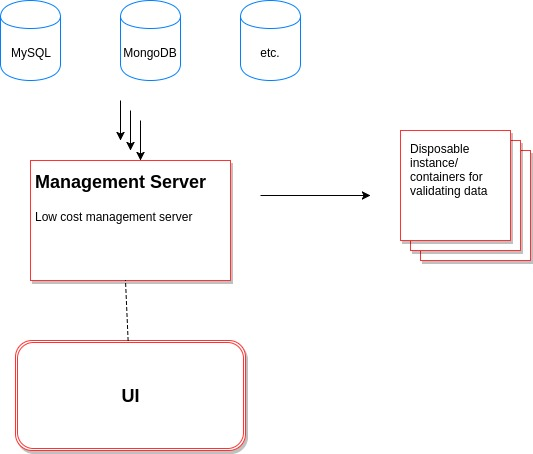
\includegraphics[width=\textwidth,height=\textheight,keepaspectratio]{diagram}
			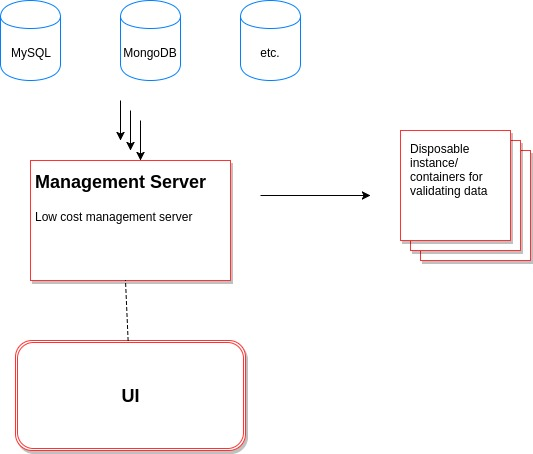
\includegraphics[scale=0.5,keepaspectratio]{diagram}
			\label{fig:diagram}
		\end{figure}
	
	\noindent \textbf{Management Server:} This will be a small low cost AWS instance on which the Jenkins automation server will be installed. The majority of the systems functionality will be carried out and/or orchestrated by this server. Jenkins jobs will copy the backups from their location to a disposable instance and implement the necessary steps to validate them such as importing and and reading.
	
	\noindent \textbf{User Interface:} This will provide a simple user interface (UI) for the system, implemented as a simple web app, hosted on AWS.It will allow users with little knowledge of Jenkins and AWS to perform backup restoration checks by adding a layer of abstraction. Users will be able to run restorations by providing the parameters such as the backup file and it's location. The UI will utilise the Jenkins API to run execute the restoration with the parameters provided.
	
	\noindent\textbf{Disposable Instances or Containers:} Disposable infrastructure will be used to perform the restoration. EC2 instances or containers can be used to quickly and easily deploy the necessary software to perform the restoration (i.e. the correct DB management system). They can also be destroyed afterwards, destroying the data and therefore maintaining confidentiality. 
	
	\subsection{Formal Modelling}
		\subsubsection{Sequence Diagrams}
		\subsubsection{User Stories}		
		\begin{tabular}{|l|p{0.4\linewidth}|p{0.4\linewidth}|} \hline
			\textbf{As a} & \textbf{I want to} & \textbf{so that} \\ \hline
			user & perform a restoration of a database backup & I can verify the backup restore process works \\ \hline
			user & view the results of a backup restore & I can verify the backup contains valid, readable data \\ \hline
			user & schedule a regular automated restoration of a particular backup & I don't have to manually do it myself \\ \hline
			user & view the results of an automated restoration check & I can verify the backup contains valid, readable data \\ \hline
			user & view past results of all automated checks & I can keep track of successful and unsuccessful restorations \\ \hline
			user & be easily notified when a restoration fail & promtly address the issue a possible backup failures \\  \hline
		\end{tabular}
	\subsection{Front End Design}
		\subsubsection{Wireframes}